\chapter{Ground Simple Action -gr}

	Action has only one effect. This effect has precondition '-1', is affecting variable with only 2 values. Then the precondition can be grounded to the other value of this variable.

	\begin{figure}
		\begin{subfigure}[b]{0.8\textwidth}
			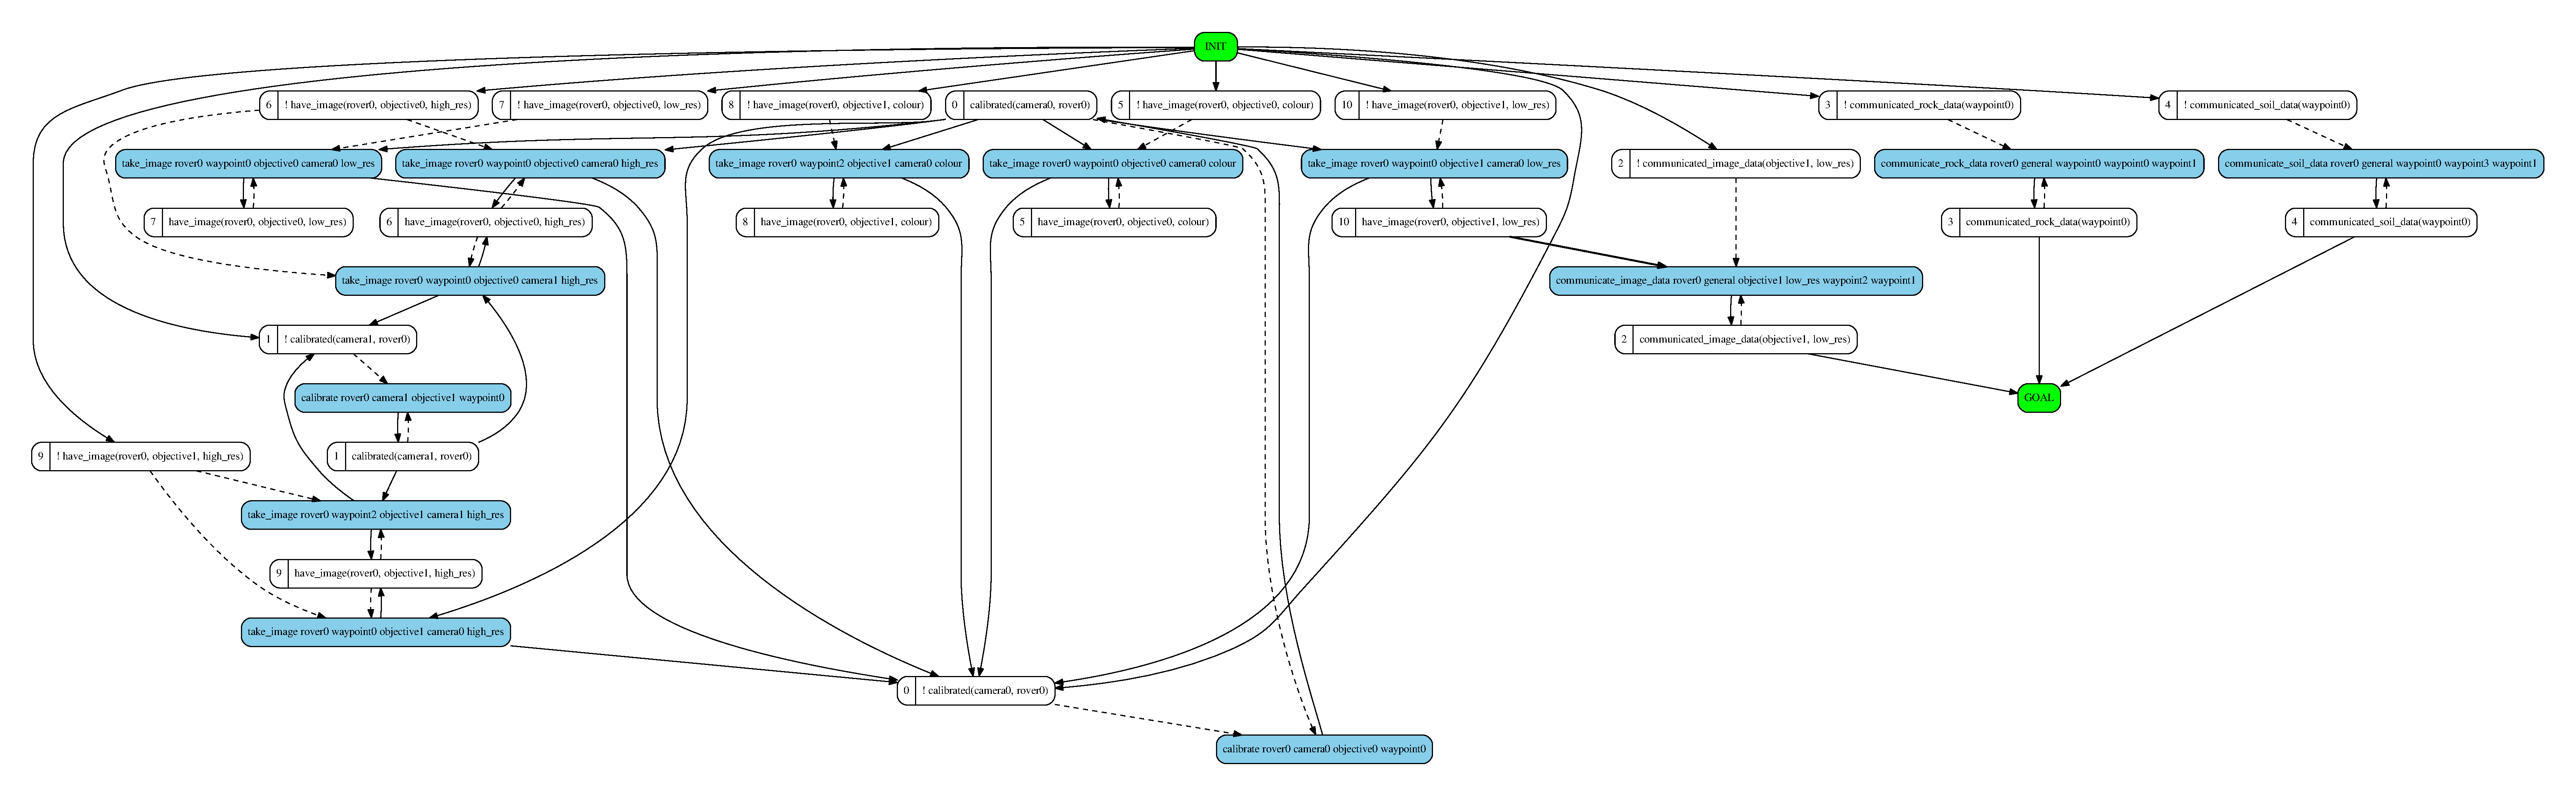
\includegraphics[width=\linewidth]{groundSimpleAction/figures/groundSimpleAction_input}
			\caption{before reduction}
		\end{subfigure}	
		
		\begin{subfigure}[b]{0.8\textwidth}
			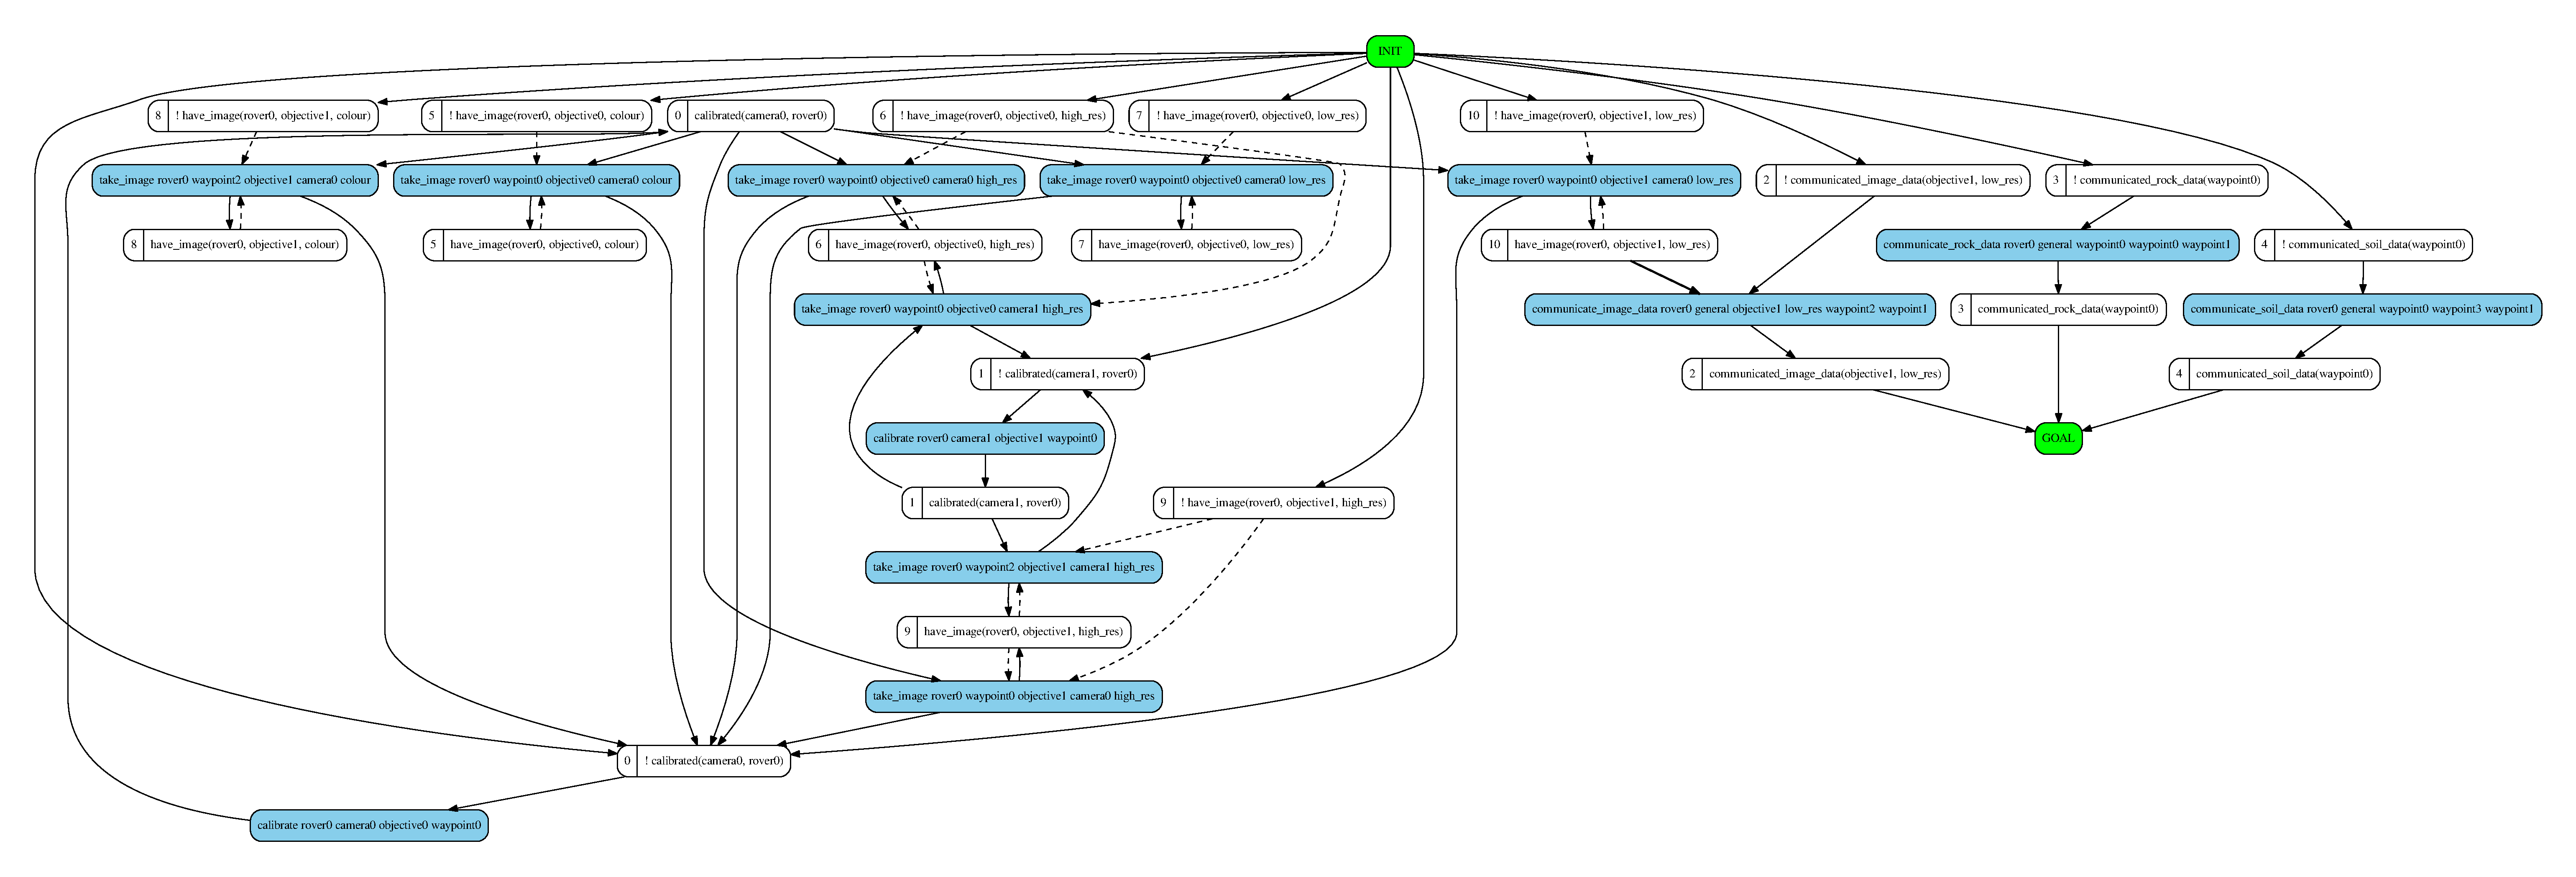
\includegraphics[width=\linewidth]{groundSimpleAction/figures/groundSimpleAction_output}
			\caption{after reduction}
		\end{subfigure}
		\caption{ }
	\end{figure}               
	
	
	\section{Reduce operation}
	
	\section{Possible outgoing states of SAS}
	\section{States before application of this operation}
	\section{Reverse operation}
	
	
	\section{Implementation notes}
	Current implementation returns MultiReverseOperation with GroundSimpleActionReverse reverse operations.